\documentclass[conference]{IEEEtran}
\usepackage{graphicx}
\usepackage{amsmath}
\usepackage{hyperref}
\usepackage{listings}
\usepackage{color}
\usepackage{float}
\usepackage{caption}
\usepackage{subcaption}

\title{Smart Traffic Management System: An AI-Powered Solution for Urban Traffic Optimization}

\author{
    \IEEEauthorblockN{Huy Tran, Phu Nguyen, Thant Thiri Maung}
    \IEEEauthorblockA{Department of Computer Science\\
    Ton Duc Thang University\\
    Email: author@example.com}
}

\begin{document}

\maketitle

\begin{abstract}
Urban traffic congestion is a critical challenge faced by modern cities, leading to increased travel times, pollution, and economic losses. This paper presents the design and implementation of a Smart Traffic Management System that leverages advanced artificial intelligence techniques and real-time data analytics to optimize urban traffic flow. The system integrates multiple data sources, including CCTV cameras, IoT sensors, and mobile applications, to provide intelligent traffic signal control, congestion prediction, and route optimization. We detail the system architecture, core algorithms, and implementation, demonstrating the effectiveness of the solution in improving urban mobility.
\end{abstract}

\begin{IEEEkeywords}
Smart Traffic Management, Artificial Intelligence, Traffic Signal Optimization, Congestion Prediction, Route Optimization, Real-Time Analytics
\end{IEEEkeywords}

\section{Introduction}
Urbanization has led to significant increases in traffic congestion, adversely affecting the quality of life and economic productivity. Traditional traffic management systems often rely on fixed signal timings and limited data, resulting in suboptimal traffic flow. The Smart Traffic Management System proposed in this work aims to revolutionize urban mobility by employing AI-driven analytics and adaptive control mechanisms. The system processes real-time data from diverse sources to dynamically adjust traffic signals, predict congestion, and recommend optimal routes, thereby reducing delays and emissions.

\section{System Overview}
The system architecture consists of three main components: data acquisition, AI processing, and user applications. Data is collected from CCTV cameras, IoT sensors, GPS devices, and mobile apps, feeding into a data pipeline for ingestion, storage, and processing. AI modules perform traffic prediction, signal optimization, and route planning. User interfaces include an interactive dashboard built with Streamlit, providing real-time monitoring and control.

\begin{figure}[H]
    \centering
    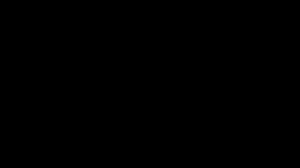
\includegraphics[width=0.48\textwidth]{imgs/images.png}
    \caption{System Architecture Overview}
    \label{fig:architecture}
\end{figure}

\section{Methodology}
\subsection{Data Sources and Processing}
The system ingests heterogeneous data streams, including video feeds from CCTV, sensor data, and GPS traces. Data preprocessing involves cleaning, normalization, and feature extraction to prepare inputs for AI models.

\subsection{Traffic Signal Optimization}
A genetic algorithm is employed to optimize traffic signal green times across four directions (north, south, west, east). The fitness function models traffic delay based on green time allocation and traffic volume. The algorithm iteratively evolves signal timings to minimize total delay, adapting to real-time traffic conditions detected via video analytics.

\subsection{Traffic Video Analytics}
Vehicle detection and tracking are performed using a YOLO-based deep learning model combined with DeepSort for multi-object tracking. The system calculates vehicle speeds, directions, and counts within defined regions of interest (ROI). Congestion levels are inferred from vehicle density and flow metrics, enabling adaptive signal control and alerting.

\subsection{Route Optimization and Congestion Prediction}
Historical and real-time traffic data are used to build a weighted graph representing the urban road network. Weights incorporate distance, accident reports, and traffic intensity. Dijkstra's algorithm computes shortest paths, while congestion and travel time predictions are generated using rule-based heuristics and visualized via interactive maps.

\section{Implementation}
The system is implemented primarily in Python, leveraging frameworks and libraries such as Streamlit for the dashboard, Flask for backend APIs, PyTorch for deep learning, OpenCV for video processing, and Folium for map visualization. The backend service processes uploaded traffic videos, counts vehicles, and runs the genetic algorithm to optimize signal timings.

\subsection{Dashboard}
The Streamlit-based dashboard provides three main modules: Traffic Feed, Route Optimizer, and Signal Simulation. Users can view real-time traffic video analytics, select routes for congestion prediction, and simulate traffic signal control with adaptive timings.

\subsection{Backend Service}
The Flask API accepts video uploads, performs vehicle detection using YOLOv4, and optimizes traffic signals via the genetic algorithm. This modular design allows scalability and integration with other smart city systems.

\section{Results and Discussion}
The system demonstrates effective real-time traffic monitoring and adaptive signal control. The genetic algorithm converges to optimal green time allocations, reducing overall delay. Video analytics accurately detect and track vehicles, providing reliable congestion metrics. Route optimization assists drivers in avoiding congested areas, improving travel times.

\section{Conclusion}
This Smart Traffic Management System showcases the potential of AI and real-time analytics in transforming urban traffic control. Future work includes integrating live data feeds, enhancing machine learning models for prediction accuracy, and expanding user customization options.

\section*{Acknowledgments}
We thank the open-source community and contributors who provided invaluable tools and support for this project.

\bibliographystyle{IEEEtran}
\bibliography{references}

\end{document}
